\newpage
\chapter{Software Architecture}
\label{chapter03}

Software development is part of the field of engineering sciences since the product is created according to the principles of building structures (in this case, software). Many decisions must be made according to the user's task when starting a new software project. This tutorial focuses on a software solution that performs parallel calculations on mobile client devices. A server assigns calculation tasks, and the resulting calculated results are received back on the same machine. On the client side, currency price values are obtained in time series form. The server also sends the artificial neural network topology information to the client. The client, in turn, uses the currency quotes and information for the artificial neural network to perform the calculations necessary to train the artificial neural network. The training process of the artificial neural network\index{artificial neural networks} is carried out using genetic algorithms\index{genetic algorithms}, which aim to find close to optimal values for the weights of the network. The client application also assumes the responsibilities of visualizing the learning process and presenting the predictions achieved. Thus shown, the system naturally leads to the choice of "client-server" software architecture.

\section{Choosing Development Tools}

In today's software industry, there is a large selection of development tools\index{development tools} for the various needs of software developers. The choice of development tools is a task in multi-criteria analysis and is mainly characterized by multiple criteria that often need revision. One part of the development tools is commercial, while another is open-source. This guide focuses primarily on open-source development tools, as minimizing production costs is a primary drive to achieve economic efficiency.

\subsection{Server Side}

For web-based server solutions, the most popular technologies are JSP, ASP, PHP, and Node.js. As ASP is a commercial technology of the Microsoft company, it is not of interest to this tutorial. JSP is a technology of the company Oracle which is open source and enables the construction of stable corporate solutions. A disadvantage of JSP is the need for more severe software and hardware resources in terms of hosting. Node.js is a technology gaining more and more popularity but has not yet reached a sufficient level of "maturity" while also requiring more software and hardware resources from the hosting side. As for PHP, the technology is narrow-purpose and has one of the highest "maturity" levels. At the same time, PHP hosting costs are among the lowest, making the choice of this technology extremely cost-effective. The task of web-based server technology is to serve as an intermediary between the network and the database management system. On the server side, storing the data in a relational database is the most rational. There are many solutions to choose from in this part of the system, the most popular being: Oracle, MS SQL Server, PostgreSQL, and MySQL. Oracle finds its application in the enterprise segment associated with high financial costs, making it unacceptable for the present aid. MS SQL Server is an alternative system to Oracle in the enterprise segment and is associated with high economic costs. PostgreSQL is an open-source system comparable to Oracle's technology capabilities and a potential candidate for low-budget development. In this manual, PostgreSQL is avoided due to its unnecessary complexity in a relatively simple software solution. The choice falls on MySQL because the system is maximally simplified, well established among users, and supported by the Oracle company. In addition to all of the above, MySQL has good support from hosting providers and is the most cost-effective choice.

\subsection{Client side}

The most common operating systems for "smart" mobile devices are Android, iOS, and Windows Phone. Microsoft has now discontinued the development of its Windows Phone operating system, which immediately leads to its rejection for the present consideration. Developing applications under iOS is cost prohibitive resulting in the dropping of this platform for the needs of this aid. Adding to the development costs is that programming for iOS is done in two languages, Objective-C and Swift, which have relatively little popularity in Eastern Europe. Most "smart" mobile devices used worldwide are with the Android operating system. Android is open source, supported mainly by Google, and allows development with significantly lower financial costs than its competitors. Android applications are primarily developed in the Java language, which is currently one of the most widely used programming languages and is characterized by a very high degree of "maturity".

\subsection{For server-client communication}

There are many possibilities for establishing communication between the server and the client. In its rawest form, information can be transmitted as a series of bytes (plain text), which leads to many difficulties in receiving and subsequent processing. A widely used alternative is the XML tag language. In this variant, the information is "packaged" in a series of tags that give a particular structure and semantics. The main intention behind the design of XML was the creation of structured documents readable by both humans and machines. For this reason, XML has a greater expressiveness than its JSON alternative. JSON is a maximally simplified tagging language for the structured representation of information, which originates from objects in the JavaScript programming language. Unlike XML, JSON is primarily intended for exchanging structured data between machines, not so much between humans and machines. Because of all of the above, in this tutorial, the choice falls on JSON as the basis for building the communication protocol between the server and its clients. Since a web-based solution is envisaged on the server side, the JSON-based protocol will run in HTTP communication sessions. For distributing web pages, the HTTP protocol was developed, using TCP/IP, to efficiently transfer information between web servers and web browsers. The HTTP protocol is well-enforced and well-supported worldwide. A critical feature of this protocol is that the communication is divided into requests and responses maintaining a single TCP/IP connection.

\section{System Components}

After a brief overview of technologies and development tools, the choice is to create a "client-server" system. The server side is responsible for data storage (MySQL database management system) and communication (PHP web scripts). The web server communicates with clients based on JSON/HTTP communication protocol. Android mobile devices make web requests, perform calculations and return the result to the server. Since it relies on donated computing power\index{donated computing resources}, choosing an appropriate way to use the mobile device without disrupting its essential functions and disturbing the users is necessary. With its Active Wallpaper technology, Android offers an ideal option for this tutorial. The active wallpaper is an image drawn behind all the main graphical components of the Android GUI. More importantly, live wallpaper is a Java application that constantly runs in the background and can perform specific short tasks when the device is not heavily loaded.

\begin{figure}[h]
\centering
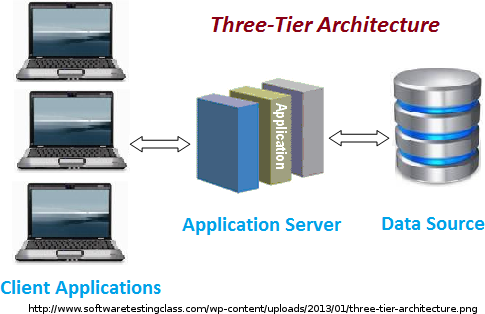
\includegraphics[width=1.0\linewidth]{pic0008}
\caption{Web-based three-tier software architecture}
\label{fig:pic0008}
\end{figure}

The choice falls on a classic three-layer software architecture when implementing the current system for distributed computing\index{distributed computing}. The same three-layer approach applies to the implementation of the mobile application, where SQLite locally stores the data being worked on, Java object-oriented code performs the calculations, and an Android-based graphical user interface takes responsibility for visualizing the process to the user.

\subsection{Development Approach}

\begin{figure}[h]
\centering
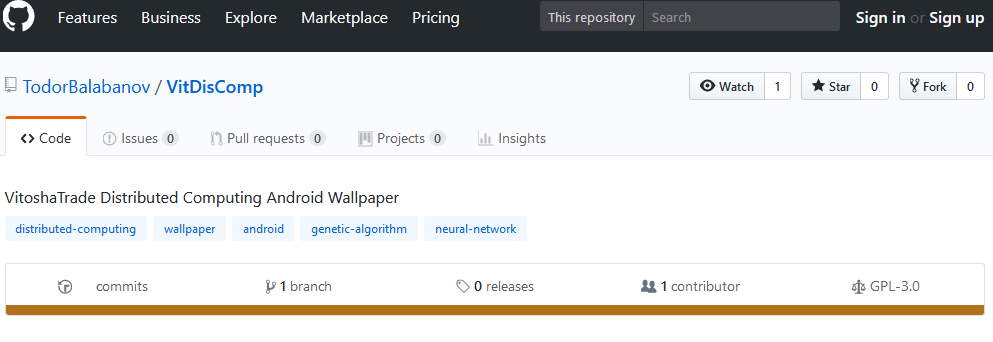
\includegraphics[width=1.0\linewidth]{pic0009}
\caption{Software Development Approaches}
\label{fig:pic0009}
\end{figure}

Assuming that the visualization is the top layer and the database is the bottom layer of a three-layer software architecture, there are two main approaches to building the software system (Fig. \ref{fig:pic0009}). In the first approach, the visual interface is first developed, then the business logic layer, and finally, the database. This approach is called "top-down" and is useful when analyzing a software job where many paper documents (sources of work screens) are already in use. This approach is also convenient for small-sized projects where the database is relatively simple. A second approach starts with the database design, then the business logic that processes the data, and finally, the screens that visualize the information. This approach is called "bottom-up" and is best suited when developing a complex software solution that is expected to work with large volumes of data and many different information structures. This tutorial focuses on the computations that mobile devices perform, not so much on creating an extensive array of data. Therefore, in this case, the choice falls on the top-down approach.

\section{Project License and Repository}

In modern open-source software projects, two things are very imortant - the legal license\index{software licenses} under which the project exists and the public repository\index{code repositories} in which the programming source code resides.

\subsection{License}

Choosing the proper software license is essential when developing a software project intended to be publicly available. There are many options, some of the most popular: a BSD License, MIT license, Mozilla Public License, and GNU General Public License. For this manual, the GNU General Public License v3 is preferred because this license is the most protective for the creator of the software product. In broad terms, GPL3 allows - commercial use, modifications, distribution, inclusion in patents, and personal use. The license carries minimal liability for the creator of the product and absolutely no guarantee of its use by users. The license also imposes a series of restrictions - mandatory inclusion of text about the authors' copyright, a list of changes made, does not allow code obfuscation, and obliges any product upgrade to be under the same license. With its protectionist nature, the GPL is one of the licenses that has given the most substantial push to the development of open-source products, which is reason enough for it to be chosen for developments without a clear commercial focus.

\subsection{Program Code Repository}

It is customary for every project to have a name, which is especially true in the world of open-source software. The name VitDisComp has been chosen for this manual. This name was chosen because the development will take advantage of the available server solution in the VIToshatrade \cite{vtrade} project, and the project is a DIStributed COMPuting solution in its essence.

\begin{figure}[h]
\centering
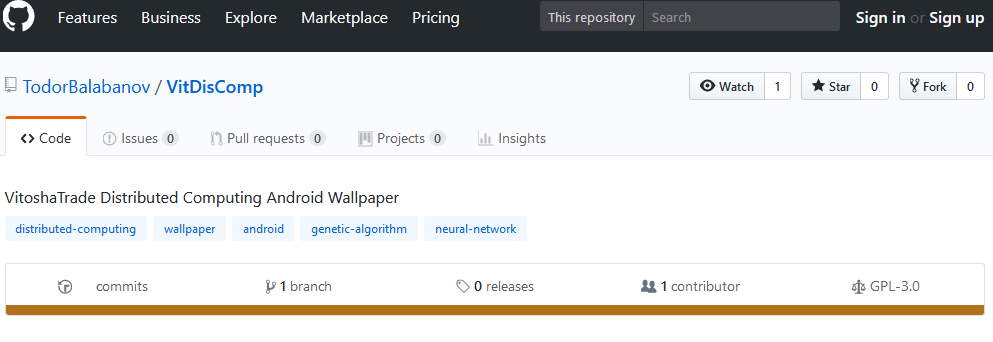
\includegraphics[width=1.0\linewidth]{pic0010}
\caption{Publish project to GitHub}
\label{fig:pic0010}
\end{figure}

There are various possibilities for publishing the program code, but one of the most popular alternatives is the cloud service GitHub. The GitHub service (Fig. \ref{fig:pic0010}) is based on the Git version control system and provides one of the most comprehensive opportunities for promoting open-license program code.
